\documentclass{sig-alternate}
\usepackage{amssymb}
\setcounter{tocdepth}{3}
\usepackage{listings}
\usepackage{booktabs}
\usepackage{mathtools}
\usepackage{tabularx}
\usepackage{fixltx2e}
\PassOptionsToPackage{hyphens}{url}\usepackage{hyperref}
\usepackage[hyphens]{url}
\usepackage{upquote,textcomp}
\lstset{breaklines=true, basicstyle=\scriptsize\ttfamily, upquote=true}

\usepackage{fancyvrb}
\VerbatimFootnotes
\usepackage{cprotect}

\usepackage{graphicx}
\makeatletter
\def\maxwidth#1{\ifdim\Gin@nat@width>#1 #1\else\Gin@nat@width\fi}
\makeatother

\usepackage{amsmath}
\usepackage{pmml-new}

\usepackage{color,graphics,array,csscolor}

\usepackage{fontspec,unicode-math}
\usepackage[Latin,Greek]{ucharclasses}
\setTransitionsForGreek{\fontspec{Times New Roman}}{}



\makeatletter
\let\@copyrightspace\relax
\makeatother
\begin{document}
\title{Generating linked RDF data from heterogeneous streaming and archival data sources: Populating the datAcron ontology.}

\numberofauthors{5}
\author{
\alignauthor
Georgios M. Santipantakis\\
\affaddr{Department of Digital Systems, School of Information and Communication Technologies, University of Piraeus, Piraeus, Greece}\\
\email{gsant@unipi.gr}
\alignauthor
George A. Vouros\\
\affaddr{Department of Digital Systems, School of Information and Communication Technologies, University of Piraeus, Piraeus, Greece}\\
\email{georgev@unipi.gr}
\alignauthor
Apostolos Glenis\\
\affaddr{Department of Digital Systems, School of Information and Communication Technologies, University of Piraeus, Piraeus, Greece}\\
\email{apostglen46@gmail.com}
\and
\alignauthor
Christos Doulkeridis\\
\affaddr{Department of Digital Systems, School of Information and Communication Technologies, University of Piraeus, Piraeus, Greece}\\
\email{cdoulk@unipi.gr}
\alignauthor
Akrivi Vlachou\\
\affaddr{Department of Digital Systems, School of Information and Communication Technologies, University of Piraeus, Piraeus, Greece}\\
\email{avlachou@aueb.gr}}
\maketitle

\begin{abstract}
Analysis of moving objects behaviour requires surveillance data (i.e. spatio-temporal data concerning objects' positional information), together with information about moving objects, occurring events and their context. Thus, data from disparate sources must be converted to a common format, integrated w.r.t. a specific model. This paper proposes a generic framework for generating RDF from heterogenous data formats - exploiting the specification of graph templates. We present and demonstrate the benefits of the proposed RDF generation process for the provision of semantically annotated data revolving around the notion of objects' trajectory. The process is demonstrated for the population of the datAcron ontology using real-world domain-specific data sources.
\end{abstract}


\category{Information systems~Resource Description Framework (RDF)}{}{}
\category{Information systems~Mediators and data integration}{}{}

\keywords{Data Integration, Heterogeneous Streaming Data, Semantic Trajectories, Triple generation}

\section{Introduction }

Monitoring and analysis of moving objects has a wide range of applications from behavioural, social and economic sciences to critical security and regulation services. This raises the need to keep track of moving objects' sequences of positions over time and annotate them with information (e.g. contextual information, information about the moving entities, and events) that may provide meaning to entities' trajectories. Trajectories are the main constructs for representing the evolution of the moving object through time and space and their annotation results to enhanced semantic (meaningful) trajectories. 

In real-life domains that are critical to our society and where trajectories are turned into ``first-class citizens'', we need a framework for the representation of moving objects' trajectories associated with varying types of information, and a method to generate RDF data from heterogeneous data sources towards providing integrated views of moving entities' data. While the first aim is achieved via the datAcron ontology proposed in  \cite{_Ref490495645}, this paper proposes a generic framework for generating RDF from heterogeneous data formats towards populating that ontology, providing examples from the maritime and aviation domains. 

In summary, this paper makes the following contributions: 
\begin{itemize}
\item Proposes a framework for generating RDF from heterogeneous sources using graph templates as a generic way to map data to RDF, supporting easy tuning of the generation process and verification of the RDF data generated; also enabling cross-data source link discovery as RDF data is generated;
\item Provides experimental results demonstrating the computational efficiency of the proposed method using real-world data sources.
\end{itemize}

\section{Requirements for RDF generation}

Although a wide range of tools have been provided for RDF generation  \cite{_Ref490495701}, the variety and heterogeneity of data associated with the construction of semantic trajectories requires a range of existing and the development of new RDF generation tools. Nevertheless, using different tools for the different data formats provided, would result to a toolset with various RDF generation tools, each with its own workflow, set-up and tuning parameters, and implementation details. In consequence, such an approach would increase the cost of maintaining the RDF generation process in its entirety, without enabling fine-grained control on the generated RDF and the links between data sets, and without enabling extensibility to data sources with new data formats and/or incorporation of changes due to changes in the ontology and in the data sources.

Concerning workflows, there should be a unique flow familiar to engineers working with RDF and SPARQL, easily instantiated and tuned to different data formats and easily verified w.r.t. the specifications of the target ontology (ontologies). The use of constructs familiar to RDF and SPARQL is important for easy adaptation to any ontology (ontologies) used and to changes to the ontologies and data sources used, enabling further verification of results.

Considering implementation, the use of different RDF generation tools hinders reusability of functions across tools (e.g. for converting data to common formats, or constructing URIs of entities), if of course they provide the flexibility to use custom functions. Using different functions in different tools, and relying on black-box solutions may result to inconsistent outputs, entailing additional, considerable cost for generating and verifying RDF data.

In addition to the above, the incorporation of streaming data provided in fast pace and big volume, require RDF generation tools that are able to consume voluminous data from high-velocity streams with the minimum possible latency.

\section{The overall RDF generation method}

The RDF generation process, shown in Figure 1, is designed in a generic way and comprises four major components: a) the data connectors, b) the triple generator, c) the integrator, and d) the triple encoder.
\begin{figure}[h!]
\centering
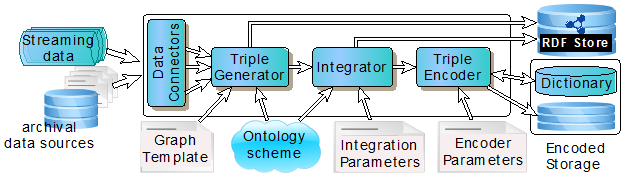
\includegraphics[width=\maxwidth{\columnwidth}]{./img/image1.png}
\cprotect\caption{  The overall RDF  generation  method .}
\label{}
\end{figure}


\subsection{Data connectors}

This component is responsible for connecting to a data source and providing access to its data. Its main task is to provide records of data from the data source to the core RDF generation component, which is the Triple Generator. 

Data connectors follow a record-by-record access model, treating both streaming and archival data sources in a uniform way: Essentially any data source is considered a ``stream'' of records that need to be processed with minimal latency. Since operations are performed on individual records, minimizing the memory footprint of the RDF generation process, also providing opportunities for scalability and parallelization (even at the level of a single data source).

The current implementation includes a variety of data connectors that support data formats: a) CSV files (surveillance, weather reports, registries of moving objects), b) direct access to databases, c) JSON messages, d) XML files, e) METAR/SPECI weather reports from offline or continuous feeds, f) National Oceanic and Atmospheric Administration (NOAA) GRIB2 files for weather reports, g) SPARQL endpoints, and h) ESRI shapefiles.

\subsection{Triple generator}

The triple generator is the core component of the RDF generation method. It converts each record provided by a data connector into a set of triples, i.e. a fragment of the RDF graph generated. This process uses two configuration files: a) a Graph Template GT, and b) a vector of variable names V. Also, the generated triples are in accordance with the datAcron ontology  \cite{_Ref490495645}, but in principle any ontology can be employed.

The Graph Template inherits the idea of standard RDF Graph Patterns, i.e. it contains triples templates, where any of the three elements in an RDF triple (s,p,o) can be a variable or a custom function. The variables and the arguments of functions are identified by a leading question mark (?), e.g. ?imo, for the IMO\footnote{ International Maritime Organization} code of a vessel, may appear as a variable in a triple or as an argument of a function. For instance the triple template:

\begin{lstlisting}[mathescape]
makeURI(?imo) rdf:type :Vessel .
\end{lstlisting}

uses the function makeURI(?imo), which constructs the URI of a resource for a given ?imo value. 

On the other hand, the vector V contains the variables that appear in the Graph Template, specifying mappings to fields in data sources.

\subsection{Integrator}

When transforming data from multiple heterogeneous sources to RDF, it is often required to link data from different sources.  The integrator is responsible for performing such a link discovery task close to the sources by identifying same entities, discovering domain-specific links among entities, and describing entities using data from different sources. 

Close to the sources link discovery is very important when entities in different sources are known to be dependent on each other, i.e. one entity exists only in relation to other entities. One such example is the case of associating weather conditions and surveillance data. Specifically, instead of transforming the entire information on weather conditions to RDF, we associate the spatio-temporal positions of moving objects trajectories with the weather variables of interest at corresponding (to those positions) spatio-temporal regions. This approach results in significant reduction of storage requirements, considering that converting a complete 3-hour weather forecast to a raw csv file requires up to 3GB of space.

Although close to the sources integration offers many benefits, it is not always applicable. For other, more complex link discovery tasks that require access to the entirety of a data source, we perform the integration independently from the RDF generation process, using blocking techniques to avoid comparisons between entities that cannot be linked.

\subsection{Triple encoder}

This component compresses the RDF triples produced by the triple generator, in order to optimize the space consumption of the RDF encoded data. It uses and maintains a dictionary for mapping URIs to unique identifiers (integer values) taking also into account spatio-temporal information.  In this way, the encoder allows applying efficient indexing techniques on top of the integer values. Details on this are omitted, as they go beyond the scope of this article.
\begin{figure}[h!]
\centering
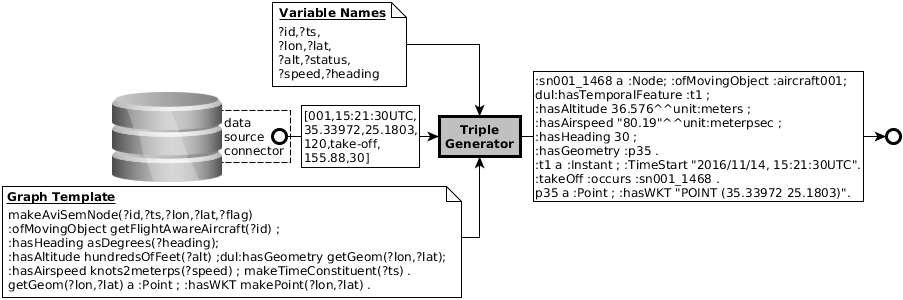
\includegraphics[width=\maxwidth{\columnwidth}]{./img/image2.png}
\cprotect\caption{  Example of RDF generation illustrating input, output, and configuration files}
\label{_Ref490495945}
\end{figure}


\section{Example on RDF generation}

A complete example of RDF generation with the corresponding configuration files is illustrated in Fig.~\ref{_Ref490495945}. The data source in this example provides surveillance data from the aviation domain that describe the spatio-temporal position of moving objects (aircrafts). The input to the triple generator is a line from a csv file, provided by the appropriate data connector. A set of eight variables is provided in order to bind input values to variable names. For example, the first variable (?id) will be bind to the first value (column) of the input record (001), and refers to the aircraft ID. The graph template constructs trajectory (semantic) nodes for aircraft, given their ID their 3-D position (?lon, ?lat and ?alt for altitude), time point (?ts), status (?status), speed (?speed) and heading (?heading). The produced output follows the structure of the graph template, after having replaced variables with the respective input values, and functions with the result of the function call. Notice that the graph template is written in compliance with the datAcron ontology  \cite{_Ref490495645}.

\section{Results on RDF generation}

Fig.~\ref{_Ref490495985} and Fig.~\ref{_Ref490495999} provide results from the RDF generation process of various real-world data sources (with data formats among those mentioned in section 3.1) in the datAcron domains. In both figures, the X-axis indicates the data source, ordered by the size of input data present in the source.

Fig.~\ref{_Ref490495985} depicts the number of raw records and the corresponding number of generated triples per data source. Notice the log scale on the y-axis. We observe that for a surveillance data source we generate 131M triples, and this corresponds to surveillance data for the maritime domain of one month.

Fig.~\ref{_Ref490495999} depicts the number of processed input records per second for the different data sources including the link discovery task, again using log scale on the y-axis. This experiment demonstrates the efficiency of the proposed RDF generation method. Focusing again on maritime surveillance data, we achieve to transform 10,467 input records to RDF per second. For some sources this number is smaller due to complicated geometries that need to be processed and advanced link discovery tasks. Overall, the average time per triple generated is approximately 0.04 seconds, given that the frequency of position reporting per aircraft/vessel is at least 2 seconds.
\begin{figure}[h!]
\centering
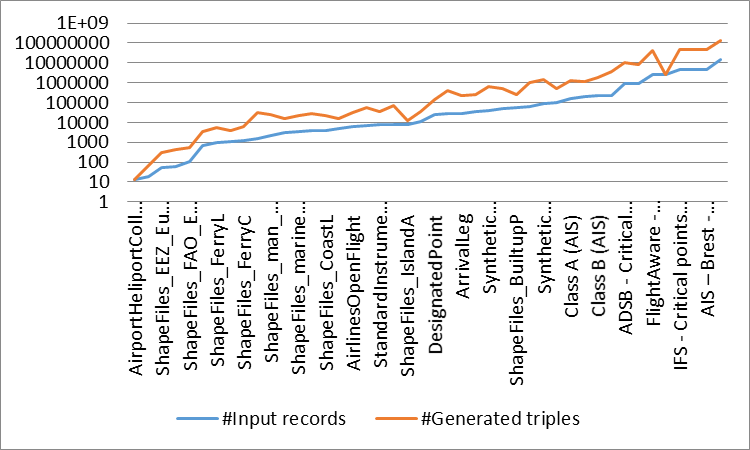
\includegraphics[width=\maxwidth{\columnwidth}]{./img/image3.png}
\cprotect\caption{  Number of input records (blue line) and generated triples (red line) per data source, ordered by number of input records in the data source}
\label{_Ref490495985}
\end{figure}

\begin{figure}[h!]
\centering
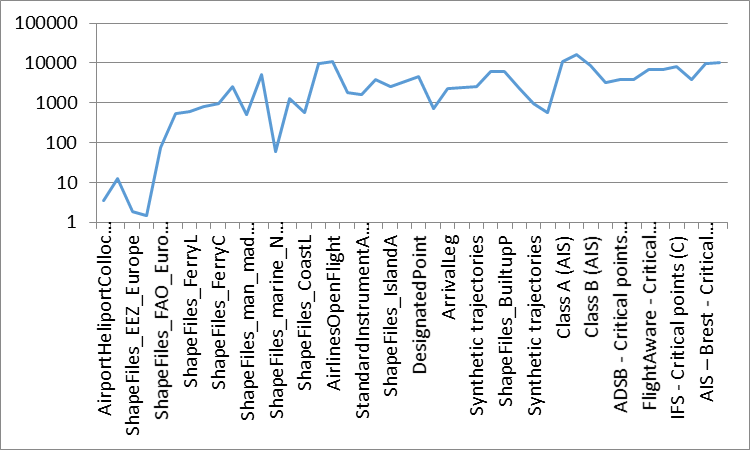
\includegraphics[width=\maxwidth{\columnwidth}]{./img/image4.png}
\cprotect\caption{  Number of generated triples per second for each data source, ordered by number of input records in the data source}
\label{_Ref490495999}
\end{figure}


\section{Concluding Remarks}

There are many RDF generators that have been developed  \cite{_Ref490495701}, most of them tailored to specific data formats (e.g. CSV, JSON, XML, XLS, etc), or even the vocabulary to be used  \cite{_Ref490495811}. Furthermore, solutions are usually tailored to a specific data format without considering the requirement for multiple source formats. The proposed approach aims to reduce the need to multiple RDF generators, providing a coherent and easy-to-be-tuned framework, further enabling its incorporation to widely used workflows, resulting to alleviating efficiency, maintenance and verification of results limitations of other approaches. Subsequent paragraphs compare our proposal with closely related works.

RDF Mapping Language (RML)  \cite{_Ref490495825} provides a mapping language for converting JSON, CSV, XML and HTML files to RDF, implemented on top of the open-source framework Sesame. RML has been proposed as an extension to R2RML  \cite{_Ref490495836}, for the conversion of RDB to RDF. Although this solution can be extensible, e.g. custom functions can be defined for data conversion, functions that enable communication between RDF generators, are difficult to be defined. Also, verification of results and maintenance can be done only by RML experts. Contrary to that, we use standard and elementary RDF constructs (graph templates) which are considerably easier to learn, maintained and incorporated into RDF and SPARQL workflows.

Datalift  \cite{_Ref490495848}, closer to our work, does not support incorporating custom functions. Datalift can parse CSV, RDF, XML, RSS, GML and ESRI shapefiles (archival sources). The assumption that the vocabulary that best describes the data is a decision of data providers is a strong assumption, since providers need agree on the related vocabularies, making also maintenance and verification of results a difficult task. 

Finally, SPARQL-Generate  \cite{_Ref490495859}, is the closest work to our proposed solution. SPARQL-Generate aims to introduce an extension to SPARQL 1.1 following the idea of SPARQL CONSTRUCT constructor, and generates triples according to a graph template. It provides constructors such as ITERATOR, useful for processing XML sources. The reliance on a SPARQL engine can introduce considerable latency issues, while only archival sources are considered. Although custom functions may be used, communication among SPARQL-Generate instances is not supported, resulting to potentially complicated workflows in cases where more than one sources are necessary to be processed concurrently.

\begin{thebibliography}{4}

\bibitem{_Ref490495836} A.Dimou, M.V.Sande, P.Colpaert, R.Verborgh, E.Mannens, and R.Van de Walle. RML: A Generic Language for Integrated RDF Mappings of Heterogeneous Data. In Proc. of WWW 2014, 2014.
\bibitem{_Ref490495701} ConverterToRdf, https://www.w3.org/wiki/ConverterToRdf , accessed 19/07/2017
\bibitem{_Ref490495848} F.Scharffe, G.Atemezing, R.Troncy, F.Gandon, S.Villata, B.Bucher, F.Hamdi, L.Bihanic, G. K\'ep\'eklian, F.Cotton, J.Euzenat, Z.Fan, P-Y.Vandenbussche, B.Vatant, Enabling linked data publication with the Datalift platform, in: Proc. AAAI workshop on semantic cities, 2012.
\bibitem{_Ref490495645} G.Santipantakis, G.A.Vouros,  C.Doulkeridis, A.Vlachou, G.Andrienko, N.Andrienko, J.M.C.Garcia, M.G.Martinez, Specification of Semantic Trajectories and Data Transformations for Analytics: The datAcron Ontology, in Proc of SEMANTICS 2017, Amsterdam, 2017.
\bibitem{_Ref490495825} M.Hert, G.Reif, and H.C.Gall. A comparison of RDB-to-RDF mapping languages. In Proc. of I-SEMANTICS 2011, 2011.
\bibitem{_Ref490495859} M.Lefrançois, A.Zimmermann, N.Bakerally, A SPARQL extension for generating RDF from heterogeneous formats, In Proc. of  ESWC 2017, 2017.
\bibitem{_Ref490495811} S.Capadisli, S.Auer, A-C.Ngonga Ngomo, Linked SDMX Data, in: Semantic Web, Linked Dataset Descriptions 2015, Volume 6, Issue 2, Pages 105 -- 112.

\end{thebibliography}

\end{document}